\documentclass[12pt,a4paper]{article}


\usepackage{amsmath,amssymb,amsfonts}
\usepackage{graphicx}
\usepackage{booktabs}
\usepackage{geometry}
\geometry{top=2.5cm, bottom=2.5cm, left=2.5cm, right=2.5cm}

\usepackage{xcolor}
\usepackage{listings}


\lstset{
    language=Matlab,
    basicstyle=\small\ttfamily,
    keywordstyle=\color{blue},
    commentstyle=\color{green!60!black},
    stringstyle=\color{orange},
    numbers=left,
    numberstyle=\tiny\color{gray},
    breaklines=true,
    frame=single,
    captionpos=b
}



\usepackage{xepersian}
\settextfont{Arial}       
\setdigitfont{Arial}      

% =========================================================
% شروع سند اصلی
% =========================================================
\begin{document}


\begin{titlepage}
    \centering
    \vspace*{2cm}
    {\Huge \bfseries گزارش کار پروژه آنالیز عددی \par}
    \vspace{1.5cm}
    
    {\large
    \vspace{0.4cm}
    \textbf{شماره گروه:} گروه 3\par
    \vspace{0.4cm}
    \textbf{اعضای گروه :} معصومه مرتضوي، شیما خلیل‌پور، ماهان رحیمی، زهرا طاهری، متین عباسی \par
    \vspace{0.4cm}
    \textbf{استاد درس:} دکتر مختاری \par
    \vspace{0.4cm}
    \textbf{تاریخ: }تیر 1405 \par
    }
    
    \vfill
    {\small دانشکده علوم ریاضی \par}
\end{titlepage}

\newpage
\tableofcontents
\newpage
% =========================================================
\section*{طرح سوال}
% =========================================================
تابع $F(x)$ به صورت زیر تعریف میشود:
\begin{equation*}
F(x) = 1 + \int_{0}^{\tan(x)}  e^{-(t-1)^2}dt , \quad x \in [0, 0.5]
\end{equation*}

\begin{enumerate}
    \item \textbf{سوال ۱ (قضیه مقدار میانگین انتگرال):} با استفاده از روش های عددی ریشه‌یابی، نقطه $c_1 \in (0,0.5)$ را تقریب بزنید به طوری که :
    \begin{equation*}
    \frac{1}{0.5-0}\int_{0}^{0.5} F(x)dx = F(c_1)
    \end{equation*}
    \item \textbf{سوال ۲ (قضیه مقدار میانگین مشتق):} با استفاده از روش های عددی ریشه‌یابی، نقطه $c_2 \in (0,0.5)$ را تقریب بزنید به طوری که :
    \begin{equation*}
    \frac{F(0.5) - F(0)}{0.5 - 0} = F'(c_2)
    \end{equation*}
\end{enumerate}

% =========================================================
\section{محاسبه تابع $F(x)$}
% =========================================================

\subsection{روش محاسبه}
برای محاسبه تقریبی تابع $F(x)$، الگوریتم دو مرحله‌ای مبتنی بر \textbf{بسط تیلور} و \textbf{انتگرال‌گیری عددی سیمپسون} به شرح زیر پیاده‌سازی شده است:

\subsubsection{مرحله اول: تقریب توابع با بسط تیلور}
اول به ازای عدد طبیعی  $n$ توابع $sin$  و $cos$ با استفاده از چند جمله ای تیلور درجه $2n+1$  و $2n$ مربوطه به صورت تقریبی محاسبه می شوند:
\begin{align*}
\sin(t) &\approx P_{\sin}(t) = t - \frac{t^3}{3!} + \frac{t^5}{5!} - \dots + (-1)^n \frac{t^{2n+1}}{(2n+1)!} \\
\cos(t) &\approx P_{\cos}(t) = 1 - \frac{t^2}{2!} + \frac{t^4}{4!} - \dots + (-1)^n \frac{t^{2n}}{(2n)!}
\end{align*}
با تقسیم این دو چندجمله‌ای، تقریبی برای تابع $\tan$ که در کران انتگرال قرار دارد به‌دست می‌آید:
\begin{equation*}
P_{\tan}(x) = \frac{P_{\sin}(x)}{P_{\cos}(x)}
\end{equation*}

همچنین برای تابع نمایی زیر انتگرال از بسط تیلور تابع $e^x$ استفاده می‌کنیم:
\begin{equation*}
e^x \approx 1 + x + \frac{x^2}{2!} + \frac{x^3}{3!} + \dots + \frac{x^k}{k!}
\end{equation*}
با جایگذاری عبارت $-(x-1)^2$ در بسط فوق، چندجمله‌ای تقریب تابع زیر انتگرال که آن را $P_f$ می‌نامیم،  که $f(x) = e^{-(x-1)^2}$،   به دست می‌آید:
\begin{equation*}
P_f(t) = 1 - (t-1)^2 + \frac{(-(t-1)^2)^2}{2!} + \frac{(-(t-1)^2)^3}{3!} + \dots + \frac{(-(t-1)^2)^k}{k!}
\end{equation*}

\subsubsection{مرحله دوم: انتگرال‌گیری عددی به روش سیمپسون}
به ازای عدد طبیعی زوج $N$،  بازه انتگرال‌گیری $[0, P_{\tan}(x)]$ را به $N$ زیربازه هم‌فاصله با طول گام $h = \frac{P_{\tan}(x)}{N}$ تقسیم می‌کنیم. گره‌های انتگرال‌گیری به صورت زیر تعریف می‌شوند:
\begin{equation*}
t_0 = 0, \quad t_i = t_0 + i \cdot h \quad (i = 0, 1, \dots, N)
\end{equation*}

در نهایت، مقدار انتگرال $F(x)$ با استفاده از فرمول سیمپسون مرکب محاسبه می‌شود:
\begin{equation*}
F(x) \approx \frac{h}{3} \left[ P_f(t_0) + 4 \sum_{i=1,3,5,\dots}^{N-1} P_f(t_i) + 2 \sum_{i=2,4,6,\dots}^{N-2} P_f(t_i) + P_f(t_N) \right]
\end{equation*} 

\subsection{  کدها و نمودارهای مربوطه}
روش فوق برای محاسبه تابع \texttt{F} در برنامه  \texttt{F.m} پیاده سازی شده و همچنین تابع به دست آمده با تابع متناظر محاسبه شده با روش های پیش‌فرض برنامه متلب مقایسه شده، که در زیر نمودار های مربوط به دو تابع در شکل \ref{comparison} و خطای میان دو تابع در شکل \ref{F_error} نمایش داده شده است; کد مربوط به رسم تصاویر در برنامه \texttt{plotting.m} ذخیره شده است.

\begin{figure}[h]
    \centering
    
\includegraphics[width=0.8\textwidth]{comparison.png}
    \caption{مقایسه تابع F محاسبه شده با روش ارائه شده و روش های پیش فرض متلب}
    \label{comparison}
\end{figure}

\begin{figure}[h]
    \centering
    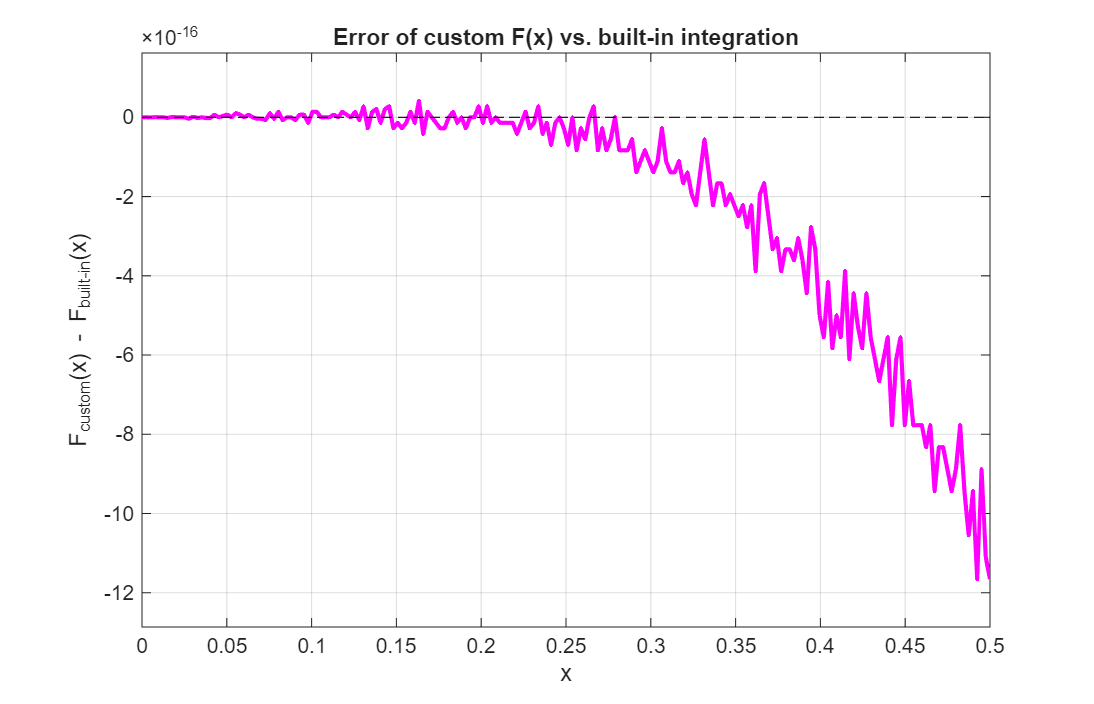
\includegraphics[width=0.8\textwidth]{F_error.png}
    \caption{خطای میان تابع F محاسبه شده با روش ارائه شده و روش های پیش فرض متلب}
    \label{F_error}
\end{figure}

\subsection{تحلیل خطای محاسبه}
در محاسبه تابع $F$ به روش فوق، سه عامل تولید خطا وجود دارد:
\begin{enumerate}
    \item \textbf{خطای تقریب تیلور در محاسبه کران انتگرال ($\tan(x)$)}
    \item \textbf{خطای تقریب تیلور تابع زیر انتگرال($e^{-(x-1)^2}$)}
    \item \textbf{خطای روش انتگرال‌گیری سیمپسون}
\end{enumerate}

\subsubsection{خظای محاسبه $\tan(x)$ :}
به ازای عدد طبیعی زوج \(n\)، اگر توابع \(P_{\sin}\) و \(P_{\cos}\) را مشابه بالا به‌ترتیب چندجمله‌ای‌های تیلورِ درجه \(2n+1\) و \(2n\) توابع \(\sin\) و \(\cos\) تعریف کنیم، آنگاه به ازای هر \(x \in [0,0.5]\)، مقادیر
\(\varepsilon_1(x)\) و \(\varepsilon_2(x)\) در بازه \((0,x)\) وجود خواهند داشت به‌طوری‌که:

\begin{gather*}
\sin(x)=P_{\sin}(x)-
\frac{\cos\bigl(\varepsilon_1(x)\bigr)}
{(2n+3)!}x^{2n+3} \ge P_{\sin}(x)-
\frac{(0.5)^{2n+3}}
{(2n+3)!} \\\\
\cos(x)=P_{\cos}(x)-
\frac{\cos\bigl(\varepsilon_2(x)\bigr)}
{(2n+2)!}x^{2n+2} \ge P_{\cos}(x)-
\frac{(0.5)^{2n+2}}
{(2n+2)!}
\end{gather*}

\vspace{0.4cm}
و در نتیجه:

\begin{gather*}
0 \le \sin(x) \le P_{\sin}(x) \le \sin(x) + \frac{(0.5)^{2n+3}}
{(2n+3)!} \\\\
0 < \cos(x) \le P_{\cos}(x) \le \cos(x) + \frac{(0.5)^{2n+2}}
{(2n+2)!}
\end{gather*}

\vspace{0.4cm}
پس:

 \begin{equation*}
 \frac{\sin(x)}{cos(x) + \frac{(0.5)^{2n+2}}{(2n+2)!}} \le 
 \frac{P_{\sin}(x)}{P_{\cos}(x)} \le
 \frac{\sin(x) + \frac{(0.5)^{2n+3}}{(2n+3)!}}{\cos(x)}
 \end{equation*}
\\
 برای سمت راست نامعادله داریم:
 \begin{align*}
     \frac{\sin(x) + \frac{(0.5)^{2n+3}}{(2n+3)!}}{\cos(x)} &=
     \tan(x) + \frac{(0.5)^{2n+3}}{(2n+3)!\cos(x)} \\\\ &\le
     \tan(x) + \frac{(0.5)^{2n+3}}{(2n+3)!\cos(0.5)} \\\\ &<
     \tan(x) + \frac{(0.5)^{2n+3}}{(2n+3)!(0.8)} \\\\ &<
     \tan(x) + \frac{5}{8}\frac{(0.5)^{2n+2}}{(2n+3)!}
 \end{align*}
 \\
 و برای سمت چپ: 
 \begin{align*}
     \frac{\sin(x)}{cos(x) + \frac{(0.5)^{2n+2}}{(2n+2)!}} &=
     \tan(x)\left( \frac{\cos(x)}{\cos(x) + \frac{(0.5)^{2n+2}}{(2n+2)!}} \right) \\\\ &=
     \tan(x)\left( 1 - \frac{\frac{(0.5)^{2n+2}}{(2n+2)!}}{\cos(x) + \frac{(0.5)^{2n+2}} {(2n+2)!}} \right) \\\\ &=
     \tan(x) - \frac{(0.5)^{2n+2}\tan(x)}{(2n+2)!\cos(x) + (0.5)^{2n+2}} \\\\ &\ge
     \tan(x) - \frac{(0.5)^{2n+2}\tan(0.5)}{(2n+2)!\cos(0.5) + (0.5)^{2n+2}} \\\\ &>
     \tan(x) - \frac{(0.5)^{2n+2}(0.6)}{(2n+2)!(0.8) + (0.5)^{2n+2}} \\\\ &>
     \tan(x) - \frac{(0.5)^{2n+2}(0.6)}{(2n+2)!(0.8)} \\\\ &=
     \tan(x) - \frac{3}{2^{2n+4}(2n+2)!}
 \end{align*}

 \newpage
 اگر مقدار بیشتر این دو کران را در نظر بگیریم، و مقدار محاسبه شده تابع $tan$(یعنی $\frac{P_{\sin}}{P_{\cos}}$) را با $P_{\tan}$ نمایش دهیم، آنگاه به ازای هر $x \in [0,0.5]$:
 
 \begin{equation}
     |P_{\tan}(x) - \tan(x)| < \frac{3}{2^{2n+4}(2n+2)!}
     \label{tan_error}
 \end{equation}

 \subsubsection{خطای محاسبه $e^{-(x-1)^2}$ :}
 
به ازای عدد طبیعی $s$، اگر $P_{f}(x)$ را مشابه بالا چندجمله‌ای تیلور درجه $s$ تابع $e^x$ در $-(x-1)^2$ تعریف کنیم، آنگاه به ازای هر $x \in [0,0.5]$، مقداری
\(\varepsilon(x)\) در بازه \((-(x-1)^2,0)\) وجود خواهد داشت به‌طوری‌که

\begin{equation*}
    e^{-(x-1)^2} = P_{f}(x) + \frac{e^{\varepsilon(x)}}{(n+1)!}
    \bigl(-(x-1)^2\bigr)^{n+1}
\end{equation*}

از آنجا که

\begin{equation*}
    -1 \le -(x-1)^2 \le -0.25,\qquad
    \varepsilon(x)\in\bigl(-(x-1)^2,0\bigr),
\end{equation*}

خواهیم داشت

\begin{equation*}
1/e < e^{\varepsilon(x)} \le 1,
\end{equation*}

و همچنین

\begin{equation*}
\bigl|-(x-1)^2\bigr|^{\,n+1}\le1.
\end{equation*}

در نتیجه،

\begin{equation}
\left|
e^{-(x-1)^2}
-
P_{\exp}\bigl(-(x-1)^2\bigr)
\right|
\le
\frac{1}{(n+1)!}.
\label{f_error}
\end{equation}

\subsubsection{خطای روش انتگرال گیری سیمپسون :}
اگر به ازای عدد طبیعی زوج ،m تابع $g \in C^4[0, 0.5]$ و $x \in [0,0.5]$، مقدار انتگرال $\int_0^xg(t)dt$ محاسبه شده با روش سیمپسون را با $S(g,x)$ نمایش دهیم، آنگاه: 
\begin{equation}
    |\int_0^xg(t)dt - S(g,x)| \le \frac{x^5 M_{g^{(4)}}}{180m^4}
    \label{simson_error}
\end{equation}

که $M_{g^{(4)}}$ کران بالایی برای مشتق چهارم $g$ است. 

\newpage
حال با در نظر گرفتن این سه مورد، با انتخاب اعداد زوج $n$ و $m$ و عدد طبیعی $s$، اگر $P_{\tan}$ و $P_f$ به نحوی که توضیح داده شد محاسبه شوند(محاسبه توابع سینوس و کسینوس تا درجه $2n+1$ و $2n$ و محاسبه تابع نمایی تا درجه $s$ چند‌جمله‌ای تیلور های مربوطه)، $S(g,x)$ مقدار $\int_0^xg(t)ft$ با روش سیمپسون مرکب با $m$ گره باشد، آنگاه به ازای $x \in [0,0.5]$، اگر قرار دهیم:

\begin{equation*}
h := \frac{P_{\tan}(x)}{m}, \quad t_0 := 0, \quad t_i := t_0 + i \cdot h \quad (i = 0, 1, \dots, N)
\end{equation*}

آنگاه:

\begin{align*}
    \left| S(P_f,P_{\tan}(x) - F(x) \right| &\le \left| S(P_f,P_{\tan}(x) - S(f,P_{\tan}(x) \right| \\\\&+
    \left| S(f,P_{\tan}(x) - \int_0^{P_{\tan}(x)}f(t)dt \right| \\\\&+
    \left| \int_0^{P_{\tan}(x)}f(t)dt - \int_0^{\tan(x)}f(t)dt \right|
\end{align*}

با استفاده از نامساوی \ref{f_error} داریم:

\begin{equation*}
    |S(P_f,P_{\tan}(x) - S(f,P_{\tan}(x)| \le \frac{P_{\tan}(x)}{(s+1)!} < \frac{0.55}{(s+1)!}
\end{equation*}

با استفاده از نامساوی \ref{simson_error} داریم: 

\begin{equation*}
    |S(f,P_{\tan}(x) - \int_0^{P_{\tan}(x)}f(t)dt| \le \frac{P_{\tan}(x)^5 M_{f^{(4)}}}{180m^4}
\end{equation*}

با استفاده از برنامه \texttt{bounds.m}، که از مشتق گیری نمادین استفاده میکند، کران $M_{f^{(4)}} = 7.42$ را برای مشتق چهارم $f$ پیدا میکنیم، و در نتیجه:

\begin{equation*}
    |S(f,P_{\tan}(x) - \int_0^{P_{\tan}(x)}f(t)dt| \le \frac{(0.55)^5 (7.42)}{180m^4} < \frac{0.00208}{m^4}
\end{equation*}

و همین‌طور با توجه به نامساوی \ref{tan_error} :

\begin{align*}
    \left| \int_0^{P_{\tan}(x)}f(t)dt - \int_0^{\tan(x)}f(t)dt \right| &= \left| \int_{\tan(x)}^{P_{\tan}(x)}f(t)dt \right| \\\\ &\le
    |P_{\tan}(x) - \tan(x)|M_{f} \\\\ &<
    |P_{\tan}(x) - \tan(x)| \\\\ &<
    \frac{3}{2^{2n+4}(2n+2)!}
\end{align*}
\\\\
با کنار هم گذاشتتن اینها: 

\begin{equation}
    |S(P_f,P_{\tan}(x) - F(x)| < \frac{0.55}{(s+1)!} + \frac{0.00208}{m^4} + \frac{3}{2^{2n+4}(2n+2)!}
    \label{F_error}
\end{equation}
\\
\textbf{مثال)}   برای نتیجه با 14 رقم با معنا(خطای کمتر از $0.5  * 10^{-14}$) کافی‌ست $n = 6$، $m = 1000$ و $s = 16$ اختیار کنیم.
\\
\textbf{توجه:} در کران خطای بدست آمده، جمله دوم(خطای ناشی از انتگرال گیری عددی) با سرعت بسیار کمتری نسبت به دو جمله دیگر کاهش پیدا میکند، در نتیجه $m$ باید نسبتا بزرگ اختیار شود، در حالی که با ثابت شدن $m$، افزایش $n$ و $s$ از حد کافی تاثیری در کران خطا نخواهد داشت.

% =========================================================
\section{سوال ۱: قضیه مقدار میانگین انتگرال}
% =========================================================

% ---------------------------------------------------------
\subsection{بررسی شرایط قضیه}
% ---------------------------------------------------------
تابع $F$ بر بازه $[0, 0.5]$ مشتق‌پذیر و در نتیجه پیوسته است؛ پس طبق قضیه مقدار میانگین برای انتگرال، نقطه $c_2 \in (0, 0.5)$ وجود دارد که:
\begin{equation*}
\frac{\int_{0}^{0.5} F(x) dx}{0.5 - 0} = F(c_2)
\end{equation*}

همین‌طور مشتق اول تابع به صورت زیر به‌دست می‌آید:
\begin{equation*}
F'(x) = e^{-(\tan(x)-1)^2} (\tan^2(x) + 1)
\end{equation*}

و از آنجایی که به ازای هر $x \in [0, 0.5]$ داریم:
\begin{equation*}
e^{-(\tan(x)-1)^2} > 0 \quad , \quad \tan^2(x) + 1 > 0
\end{equation*}

پس تابع $F'$ در بازه $[0, 0.5]$ مثبت است، و در نتیجه تابع $F$ در این بازه \textbf{اکیداً صعودی} است. بنابراین نقطه $c_2$ با شرایط فوق \textbf{یکتا} است.


% ---------------------------------------------------------
\subsection{روش حل سوال}
% ---------------------------------------------------------
اول با استفاده از روش سیمپسون، مقدار انتگرال $\int_{0}^{0.5} F(x) dx$ را محاسبه می‌کنیم و مقدار میانگین انتگرال $F$ را به طور تقریبی به‌دست می‌آوریم:
\begin{equation*}
A := \frac{\int_{0}^{0.5} F(x) dx}{0.5 - 0} \approx 1.133295976021740
\end{equation*}

برای حل سوال از ترکیبی از دو روش **دوبخشی (Bisection)** و **تکرار ساده (Fixed-Point Iteration)** استفاده شده است. ابتدا پنج مرحله از روش دوبخشی انجام شده تا به بازه‌ای کوچک‌تر شامل $c_2$ دست یابیم، که نتایج آن به صورت جدول \ref{tab:bisection_steps} بود:

\begin{table}[h]
\centering
\caption{مراحل روش دوبخشی برای رسیدن به تقریب اولیه $c_2$}
\label{tab:bisection_steps}
\vspace{0.2cm}
\begin{tabular}{cc}
\toprule
\textbf{بازه} & \textbf{نقطه وسط} \\
\midrule
$[0, 1/2]$ & $1/4$ \\
$[1/4, 1/2]$ & $3/8$ \\
$[1/4, 3/8]$ & $5/16$ \\
$[1/4, 5/16]$ & $9/32$ \\
$[1/4, 9/32]$ & $17/64$ \\
$[17/64, 9/32]$ & $35/128$ \\
\bottomrule
\end{tabular}
\end{table}

\newpage
و در نتیجه به تقریب اولیه از $c_2$ یعنی $\frac{35}{128}$ رسیده‌ایم. از این تقریب برای تعریف تابع $g(x)$ برای الگوریتم تکرار ساده استفاده می‌کنیم. قرار می‌دهیم:
\begin{equation*}
g_m(x) := x - m(F(x) - A)
\end{equation*}
که واضح است به ازای هر $m \neq 0$، و هر $x$، $x$ نقطه ثابت $g_m$ است اگر و تنها اگر $F(x) = A$ باشد.

حال $m$ را طوری انتخاب می‌کنیم که $|g_m'(x)|$ تا حد امکان کوچک شود (دلایل مربوطه در بخش تحلیل خطا). اما چون:
\begin{equation*}
g_m'(x) = 1 - m F'(x)
\end{equation*}
یک انتخاب خوب می‌تواند $m = \frac{1}{F'(c_2)}$ باشد که در این صورت $g_m'$ در $c_2$ صفر شده و در نتیجه در بازه کوچکی اطراف آن بسیار کوچک خواهد بود.

اما چون به $c_2$ دسترسی نداریم، از تقریب اولیه به‌دست آمده استفاده می‌کنیم و مقدار $m := \frac{1}{F'(\frac{35}{128})}$ و تابع زیر را قرار می‌دهیم:
\begin{equation*}
g(x) := x - \frac{F(x) - A}{F'\left(\frac{35}{128}\right)}
\end{equation*}

مقدار $F'\left(\frac{35}{128}\right)$ را با استفاده از روش مشتق‌گیری عددی سه نقطه‌ای مرکزی تقریب می‌زنیم که به ازای $h = \frac{0.5}{1000}$ به نتیجه زیر می‌رسیم:
\begin{equation*}
F'\left(\frac{35}{128}\right) \approx \frac{F\left(\frac{35}{128} + h\right) - F\left(\frac{35}{128} - h\right)}{2h} \approx 0.642741
\end{equation*}
و در نتیجه:
\begin{equation*}
m = \frac{1}{F'\left(\frac{35}{128}\right)} \approx 1.55584
\end{equation*}

حال با استفاده از تابع $g$ و نقطه شروع $\frac{35}{128}$، شش مرحله از روش تکرار ساده را پیاده‌سازی می‌کنیم و به نتایج جدول \ref{tab:fixed_point_results} می‌رسیم:

\begin{table}[h!]
\centering
\caption{نتایج شش مرحله از روش تکرار ساده برای محاسبه $c_2$}
\label{tab:fixed_point_results}
\vspace{0.2cm}
\begin{tabular}{cc}
\toprule
\textbf{تکرار ($k$)} & \textbf{مقدار $x_k$} \\
\midrule
۱ & $0.271824116420384$ \\
۲ & $0.271821369353568$ \\
۳ & $0.271821359997641$ \\
۴ & $0.271821359965749$ \\
۵ & $0.271821359965640$ \\
۶ & $0.271821359965640$ \\
\bottomrule
\end{tabular}
\end{table}


\subsection{کدها، نمودارها و نتایج به‌دست آمده}
کد متلب مربوط به ریشه‌یابی:
\textbf{توجه:} کد مربوطه در برنامه \texttt{derivative\_mvt.m} ذخیره شده است.




% ---------------------------------------------------------
\subsection{تحلیل خطای روش}
% ---------------------------------------------------------
در این بخش به تحلیل خطای روش و اینکه آیا اصلاً تابع $g$ تعریف شده در شرایط قضیه نقطه ثابت صدق می‌کند یا خیر می‌پردازیم.

تابع $g(x)$ را در بازه $\left[\frac{17}{64}, \frac{18}{64}\right]$ که از طریق روش دوبخشی به‌دست آورده‌ایم در نظر می‌گیریم. 

چون مشتق دوم تابع $F$ در بازه تعریف مثبت است، در نتیجه $F'$ اکیداً صعودی بوده و به ازای هر $x \in \left[\frac{17}{64}, \frac{18}{64}\right]$ داریم:
\begin{equation}
F'\left(\frac{17}{64}\right) \le F'(x) \le F'\left(\frac{18}{64}\right)
\end{equation}

و در نتیجه برای مشتق $g'(x)$ خواهیم داشت:
\begin{equation*}
1 - m F'\left(\frac{18}{64}\right) \le g'(x) \le 1 - m F'\left(\frac{17}{64}\right)
\end{equation*}

که با محاسبه عددی حدود این مقادیر به نابرابری‌های زیر می‌رسیم:
\begin{equation*}
-0.01667 < 1 - m F'\left(\frac{18}{64}\right) < 0 < 1 - m F'\left(\frac{17}{64}\right) < 0.01636
\end{equation*}

بنابراین به ازای هر $x \in \left[\frac{17}{64}, \frac{18}{64}\right]$ داریم:
\begin{equation*}
|g'(x)| < 0.01667
\end{equation*}

همین‌طور برای مشتق دوم تابع $g$ داریم:
\begin{equation*}
g''(x) = -m F''(x)
\end{equation*}

از آنجایی که $F''$ در بازه همواره مثبت است، پس $g''$ در این بازه منفی بوده و در نتیجه $g'$ در بازه اکیداً نزولی است. همچنین چون $g'\left(\frac{17}{64}\right) > 0$ و $g'\left(\frac{18}{64}\right) < 0$، پس $g'$ در بازه دقیقاً یک ریشه دارد که آن ریشه، نقطه ماکزیمم $g$ در بازه است. این نقطه را با روش دوبخشی تقریب می‌زنیم:
\begin{equation*}
x_{max} \approx 0.273437501872005 \quad,\quad g(x_{max}) \approx 0.271824116420395
\end{equation*}

و مقادیر تابع $g$ در دو انتهای بازه به صورت زیر است:
\begin{align*}
g\left(\frac{17}{64}\right) &\approx 0.271824116420395 < 0.271825 \\
g\left(\frac{18}{64}\right) &\approx 0.271759215532293 > 0.27175
\end{align*}

پس به ازای هر $x \in \left[\frac{17}{64}, \frac{18}{64}\right]$ داریم:
\begin{equation*}
\frac{17}{64} < 0.27175 < g(x) < 0.271825 < \frac{18}{64} \implies g\left(\left[\frac{17}{64}, \frac{18}{64}\right]\right) \subseteq \left[\frac{17}{64}, \frac{18}{64}\right]
\end{equation*}
بنابراین تابع $g$ در شرایط **قضیه نقطه ثابت (Fixed-Point Theorem)** صدق می‌کند.

همچنین با توجه به قضایای خطای روش تکرار ساده و به ازای تقریب‌های $x_i$ به‌دست آمده با نقطه آغاز $\frac{35}{128}$، به ازای هر تکرار $i$ رابطه خطای زیر برقرار است:
\begin{equation*}
|x_i - c_2| \le M_{g'}^i \cdot \left(\frac{1}{128}\right) < \frac{(0.01667)^i}{128}
\end{equation*}
که در آن $M_{g'}$ کران بالایی مشتق $|g'|$ است.

برای مثال به ازای $i = 6$ مرحله تکرار داریم:
\begin{equation*}
|x_6 - c_2| < 1.68 \times 10^{-13}
\end{equation*}
بنابراین حداقل تا **۱۲ رقم با‌معنا** دقت انتظار می‌رود.

% =========================================================
\section{سوال ۲: قضیه مقدار میانگین مشتق}
% =========================================================
% ---------------------------------------------------------
\subsection{بررسی شرایط قضیه}
% ---------------------------------------------------------
برای بررسی شرایط قضیه و اثبات وجود و یکتایی نقطه $c$، ابتدا وجود چنین نقطه‌ای را بررسی می‌کنیم:

\begin{itemize}
    \item تابع $e^{-(t-1)^2}$ روی $\mathbb{R}$ پیوسته است، در نتیجه طبق قضیه اساسی حساب، تابع زیر نسبت به $x$ مشتق‌پذیر است و داریم:
    \begin{equation*}
    \left(\int_{0}^{x} e^{-(t-1)^2} dt\right)' = e^{-(x-1)^2}
    \end{equation*}

    همچنین تابع $\tan(x)$ روی بازه $[0, 0.5]$ مشتق‌پذیر است و $(\tan(x))' = 1 + \tan^2(x)$ روی $(0, 0.5)$ است.

    \item پس طبق قضیه مشتق زنجیره‌ای، تابع $F(x)$ مشتق‌پذیر بوده و مشتق آن برابر است با:
    \begin{equation*}
    F'(x) = e^{-(\tan(x)-1)^2} \cdot (1 + \tan^2(x))
    \end{equation*}
\end{itemize}

بنابراین تابع بر بازه $[0, 0.5]$ پیوسته و بر $(0, 0.5)$ مشتق‌پذیر است، پس طبق قضیه مقدار میانگین، نقطه $c \in (0, 0.5)$ وجود دارد که:
\begin{equation*}
F'(c) = \frac{F(0.5) - F(0)}{0.5 - 0}
\end{equation*}

\begin{itemize}
    \item همین‌طور طبق قضایای مشتق، تابع $F'$ روی $(0, 0.5)$ مشتق‌پذیر است و اگر قرار دهیم:
    \begin{equation*}
    g(x) := \left(e^{-(\tan(x)-1)^2}\right)' = -2e^{-(\tan(x)-1)^2}(\tan(x) - 1)(1 + \tan^2(x))
    \end{equation*}

    آنگاه مشتق دوم $F''(x)$ به صورت زیر به‌دست می‌آید:
    \begin{equation*}
    F''(x) = g(x) + g(x) \tan^2(x) + 2e^{-(\tan(x)-1)^2} \tan(x) = (1 + \tan^2(x)) \cdot \left[ g(x) + 2e^{-(\tan(x)-1)^2} \cdot \tan(x) \right]
    \end{equation*}
\end{itemize}

عبارات $e^{-(\tan(x)-1)^2}$ و $(1 + \tan^2(x))$ کلاً روی $\mathbb{R}$ مثبت هستند و عبارت $1 - \tan(x)$ در $[0, 0.5]$ مثبت است، در نتیجه $g(x)$ در $[0, 0.5]$ مثبت است. همین‌طور $\tan(x)$ در $(0, 0.5)$ مثبت است و در نتیجه $F''(x)$ در $(0, 0.5)$ مثبت بوده و تابع $F'$ در بازه $[0, 0.5]$ **اکیداً صعودی** می‌باشد.

پس نقطه یکتای $c \in (0, 0.5)$ موجود است که:
\begin{equation*}
F'(c) = \frac{F(0.5) - F(0)}{0.5 - 0}
\end{equation*}


% ---------------------------------------------------------
\subsection{روش حل سوال}
% ---------------------------------------------------------
نقاط $x_i$ از بازه مربوطه را به طور دلخواه انتخاب می‌کنیم و به ازای مقدار مثبت کوچک $h$، به ازای هر $x_i$، مقدار تقریبی مشتق $F$ در $x_i$ را با \textbf{روش سه نقطه‌ای مرکزی} محاسبه می‌کنیم:
\begin{equation*}
y_i := \frac{F(x_i+h) - F(x_i-h)}{2h}
\end{equation*}

تابع درون‌یاب $P(x)$ گذرنده از نقاط $(x_i, y_i)$ را با \textbf{روش لاگرانژ} محاسبه می‌کنیم. این تابع تقریباً برای تابع $F'(x)$ در بازه مربوطه است.

قرار می‌دهیم:
\begin{equation*}
m := \frac{F(0.5) - F(0)}{0.5 - 0}
\end{equation*}

اگر خطای میان $P(x)$ تا حد کافی کوچک باشد، آنگاه $(P(0) - m)(P(0.5) - m) < 0$ خواهد بود و در نتیجه تابع $P(x) - m$ در بازه حداقل یک ریشه خواهد داشت. با استفاده از \textbf{روش دو بخشی} یک چنین ریشه‌ای را به طور تقریبی محاسبه می‌کنیم و نقطه بدست آمده را به عنوان تقریبی برای $c$ در نظر می‌گیریم.

% ---------------------------------------------------------
\subsection{کدها، نمودارها و نتایج به‌دست آمده}
% ---------------------------------------------------------
روش فوق به ازای $n = 20$ نقاط هم‌فاصله در برنامه \texttt{derivative\_mvt.m} پیاده‌سازی شده و در آخر هم با استفاده از روش دو بخشی تا ۸ رقم با معنا محاسبه شده و نتیجه زیر حاصل شده است:
\begin{equation*}
c = 0.27492790
\end{equation*}
نمودار مربوط به برنامه بالا، شامل نقاط انتخاب شده، مقادیر مشتق محاسبه شده، منحنی درون‌یاب گذرنده از آن‌ها و نقطه $c$ پیدا شده در شکل \ref{fig:derivative_plot} نشان داده شده و کد مربوط به رسم آن در برنامه \texttt{Plotting.m} ذخیره شده است.

\begin{figure}[h!]
    \centering
    
\includegraphics[width=0.6\textwidth]{derivative_mvt.png}
 
    \caption{نمودار مشتق عددی $F'(x_i)$، منحنی درون‌یاب لاگرانژ $P(x)$ و تعیین نقطه $(c, P(c))$}
    \label{fig:derivative_plot}
    \label{fig:derivative_plot}
\end{figure}


\end{document}